\begin{figure}[h]
\begin{lstc}
#define CPUID_GETFEATURES 0x00000001
#define CPUID_FEAT_EDX_TSC (1 << 4)
...
__asm__ volatile ("cpuid" :
    "=a" (regs->rax),
    "=b" (regs->rbx),
    "=c" (regs->rcx),
    "=d" (regs->rdx)
    : "a" (CPUID_GETFEATURES), "c" (0));

tsc  = (regs->rdx & CPUID_FEAT_EDX_TSC);

if (!tsc) printf("detected ether!\n");
\end{lstc}
\caption{\label{fig:cpuid-tsc} Code snippet in C showing how to check for TSC
  support through the CPUID instruction.}
\end{figure}

\begin{figure*}[!t]
	\centering
	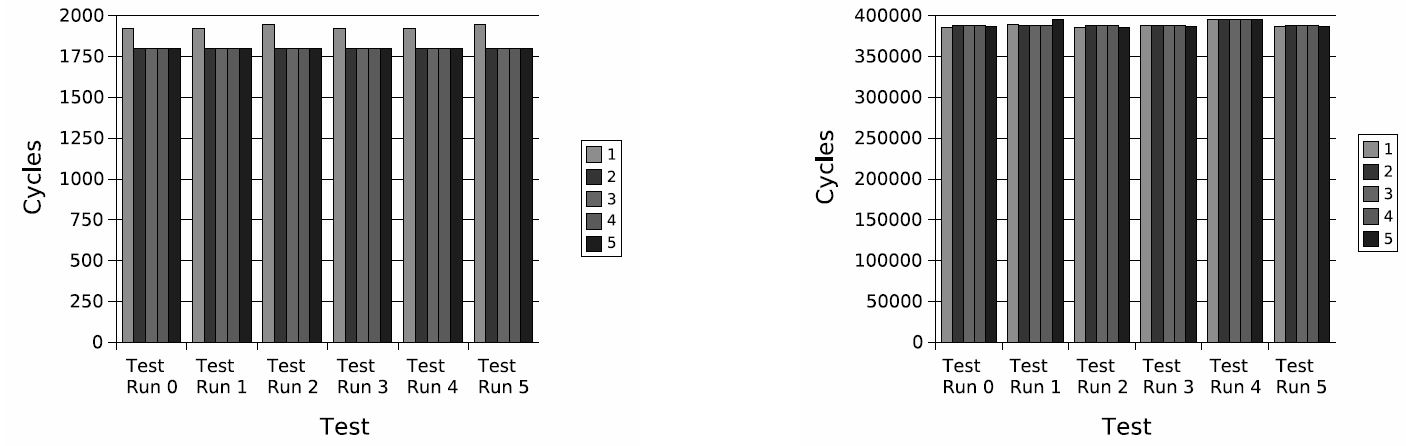
\includegraphics[width=\textwidth]{figure/realhw.jpg}
	\caption{Real hardware Cache On (left), Cache Off (right)}
	\label{fig:cache_realhw}
\end{figure*}

\begin{figure*}[!t]
	\centering
	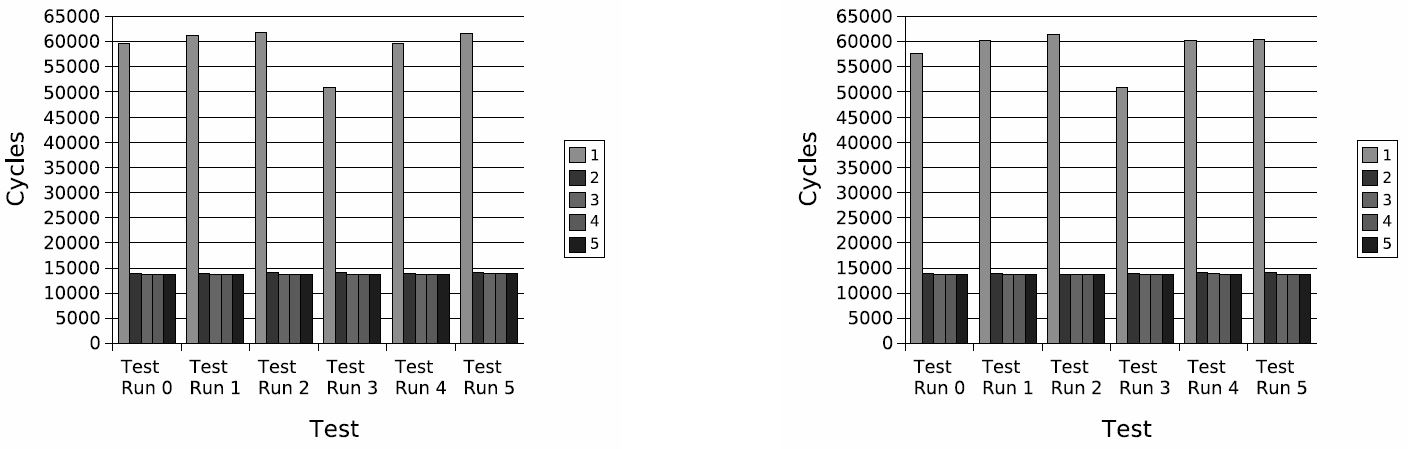
\includegraphics[width=\textwidth]{figure/qemu.jpg}
	\caption{Qemu On (left), Cache Off (right)}
	\label{fig:cache_qemu}
\end{figure*}

\begin{figure*}[!t]
	\centering
	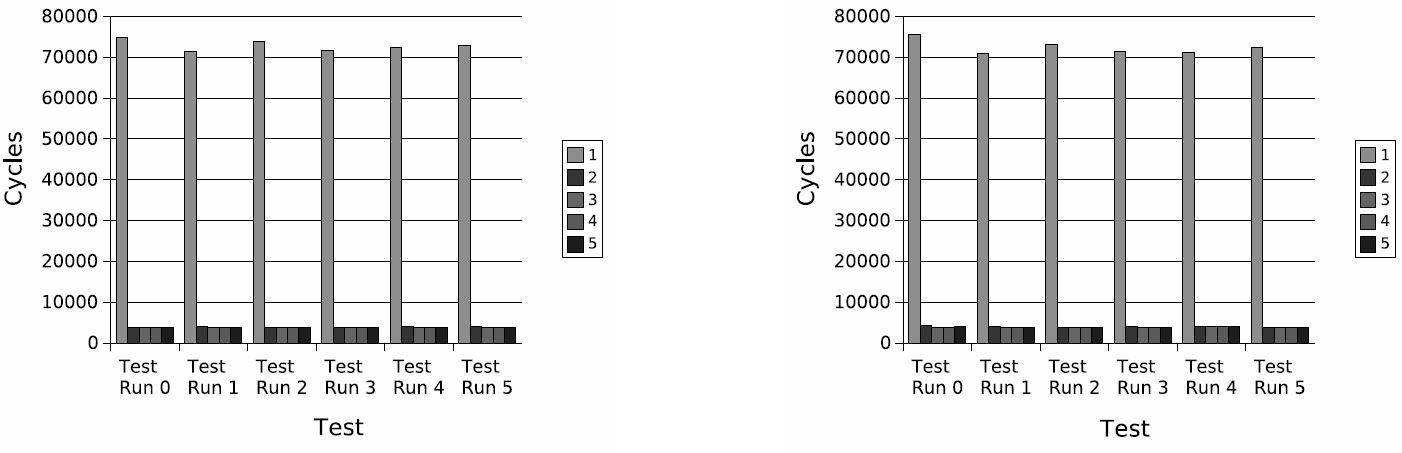
\includegraphics[width=\textwidth]{figure/vmware.jpg}
	\caption{VMware Cache On (left), Cache Off (right)}
	\label{fig:cache_vmware}
\end{figure*}

%%% Local Variables:
%%% mode: latex
%%% TeX-master: "../paper"
%%% End:
